\documentclass[utf8,hyperref={colorlinks=true}]{beamer}
\definecolor{links}{HTML}{2A1B81}
\hypersetup{colorlinks,linkcolor=,urlcolor=links}
\mode<presentation>
\usepackage{multicol}
\usepackage{listings}
\usepackage{helvet}
\usepackage{tikz}
\usetheme{Warsaw}
\usecolortheme{whale}
\usefonttheme[onlylarge]{structuresmallcapsserif}
\usefonttheme[onlysmall]{structurebold}
\usepackage{amsthm} % pushQED, popQED
\newenvironment{aquote}[1]{%
  \pushQED{#1}%
  \begin{quote}
}{%
  \par\noindent\hfill(\popQED)%
  \end{quote}%
}

\setbeamercovered{dynamic}
\setbeameroption{show notes}

\makeatletter
\newenvironment{btHighlight}[1][]
{\begingroup\tikzset{bt@Highlight@par/.style={#1}}\begin{lrbox}{\@tempboxa}}
{\end{lrbox}\bt@HL@box[bt@Highlight@par]{\@tempboxa}\endgroup}

\newcommand\btHL[1][]{%
  \begin{btHighlight}[#1]\bgroup\aftergroup\bt@HL@endenv%
}
\def\bt@HL@endenv{%
  \end{btHighlight}%   
  \egroup
}
\newcommand{\bt@HL@box}[2][]{%
  \tikz[#1]{%
    \pgfpathrectangle{\pgfpoint{1pt}{0pt}}{\pgfpoint{\wd #2}{\ht #2}}%
    \pgfusepath{use as bounding box}%
    \node[anchor=base west, fill=orange!30,outer sep=0pt,inner xsep=1pt, inner ysep=0pt, rounded corners=3pt, minimum height=\ht\strutbox+1pt,#1]{\raisebox{1pt}{\strut}\strut\usebox{#2}};
  }%
}
\makeatother

\begin{document}
\title{Tu primer servidor en Erlang con SSE}
\subtitle{utilizando Cowboy y Sumo DB}
\author{Fernando Benavides (\textit{@elbrujohalcon})}
\institute{Inaka Labs}
\date{\today}
\logo{
\includegraphics[height=0.5cm]{img/inaka-logo.png}}

\newcommand*\oldmacro{}%
\let\oldmacro\insertshorttitle%
\renewcommand*\insertshorttitle{%
  \oldmacro\hfill%
  \insertframenumber\,/\,\inserttotalframenumber}

%%%%%%%%%%%%%%%%%%%%%%%%%%%%%%%%%%%%%%%%%%%%%%%%%%%%%%%%%%%%%%%%%%%%%%
%% CODE SNIPPETS
%%%%%%%%%%%%%%%%%%%%%%%%%%%%%%%%%%%%%%%%%%%%%%%%%%%%%%%%%%%%%%%%%%%%%%
\definecolor{darkblue}{rgb}{0,0.08,0.45} 

\lstset{% general command to set parameter(s)
		mathescape=true,
		language=erlang,
		basicstyle=\ttfamily\scriptsize,
		keywordstyle=\color{blue}\bfseries,
		identifierstyle=\color{darkblue},
		stringstyle=\ttfamily,
		moredelim=**[is][{\btHL[fill=green!30,draw=red,dashed,thin]}]{@}{@},
		showstringspaces=false}

\defverbatim[colored]\handlerinit{%
\begin{lstlisting}[frame=single]
init(_Transport, Req, _Opts) ->
  case cowboy_req:method(Req) of
    {<<"POST">>, _} ->
      {upgrade, protocol, cowboy_rest};
    {<<"GET">>, Req1} ->
      handle_get(Req1)
  end.
\end{lstlisting}
}

\defverbatim[colored]\restcallbacks{%
\begin{lstlisting}[frame=single]
allowed_methods(Req, State) ->
  {[<<"POST">>], Req, State}.

content_types_accepted(Req, State) ->
  {[{<<"application/json">>, handle_post}], Req, State}.

resource_exists(Req, State) ->
  {false, Req, State}.
\end{lstlisting}
}

\defverbatim[colored]\restcallbacksa{%
\begin{lstlisting}[frame=single]
allowed_methods(Req, State) ->
  {[<<"POST">>], Req, State}.

content_types_accepted(Req, State) ->
  {[{<<"application/json">>, @handle_post@}], Req, State}.

resource_exists(Req, State) ->
  {false, Req, State}.
\end{lstlisting}
}

\defverbatim[colored]\handlepost{%
\begin{lstlisting}[frame=single]
handle_post(Req, State) ->
  {ok, Body, Req1} = cowboy_req:body(Req),
  case json_decode(Body) of
    {Params} ->
      Title =
        proplists:get_value(<<"title">>, Params, <<"News">>),
      Content =
        proplists:get_value(<<"content">>, Params, <<"">>),
      NewsFlash = canillita_news:new(Title, Content),
      notify(NewsFlash),
      {true, Req1, State};
    {bad_json, Reason} ->
      {ok, Req2} =
        cowboy_req:reply(400,[],jiffy:encode(Reason),Req1),
      {halt, Req2, State}
  end.
\end{lstlisting}
}

\defverbatim[colored]\handleposta{%
\begin{lstlisting}[frame=single]
handle_post(Req, State) ->
  @{ok, Body, Req1} = cowboy_req:body(Req),@  
  case json_decode(Body) of
    {Params} ->
      Title =
        proplists:get_value(<<"title">>, Params, <<"News">>),
      Content =
        proplists:get_value(<<"content">>, Params, <<"">>),
      NewsFlash = canillita_news:new(Title, Content),
      notify(NewsFlash),
      {true, Req1, State};
    {bad_json, Reason} ->
      {ok, Req2} =
        cowboy_req:reply(400,[],jiffy:encode(Reason),Req1),
      {halt, Req2, State}
  end.
\end{lstlisting}
}

\defverbatim[colored]\handlepostb{%
\begin{lstlisting}[frame=single]
handle_post(Req, State) ->
  {ok, Body, Req1} = cowboy_req:body(Req),
  @case json_decode(Body) of@
   @ {Params} ->@
      Title =
        proplists:get_value(<<"title">>, Params, <<"News">>),
      Content =
        proplists:get_value(<<"content">>, Params, <<"">>),
      NewsFlash = canillita_news:new(Title, Content),
      notify(NewsFlash),
      {true, Req1, State};
    @{bad_json, Reason} ->@
      {ok, Req2} =
        cowboy_req:reply(400,[],jiffy:encode(Reason),Req1),
      {halt, Req2, State}
  @end@.
\end{lstlisting}
}

\defverbatim[colored]\handlepostc{%
\begin{lstlisting}[frame=single]
handle_post(Req, State) ->
  {ok, Body, Req1} = cowboy_req:body(Req),
  case json_decode(Body) of
    {Params} ->
      @Title =@
        @proplists:get_value(<<"title">>, Params, <<"News">>),@
      @Content =@
        @proplists:get_value(<<"content">>, Params, <<"">>)@,
      NewsFlash = canillita_news:new(Title, Content),
      notify(NewsFlash),
      {true, Req1, State};
    {bad_json, Reason} ->
      {ok, Req2} =
        cowboy_req:reply(400,[],jiffy:encode(Reason),Req1),
      {halt, Req2, State}
  end.
\end{lstlisting}
}

\defverbatim[colored]\handlepostd{%
\begin{lstlisting}[frame=single]
handle_post(Req, State) ->
  {ok, Body, Req1} = cowboy_req:body(Req),
  case json_decode(Body) of
    {Params} ->
      Title =
        proplists:get_value(<<"title">>, Params, <<"News">>),
      Content =
        proplists:get_value(<<"content">>, Params, <<"">>),
      @NewsFlash = canillita_news:new(Title, Content),@
      notify(NewsFlash),
      {true, Req1, State};
    {bad_json, Reason} ->
      {ok, Req2} =
        cowboy_req:reply(400,[],jiffy:encode(Reason),Req1),
      {halt, Req2, State}
  end.
\end{lstlisting}
}

\defverbatim[colored]\handleposte{%
\begin{lstlisting}[frame=single]
handle_post(Req, State) ->
  {ok, Body, Req1} = cowboy_req:body(Req),
  case json_decode(Body) of
    {Params} ->
      Title =
        proplists:get_value(<<"title">>, Params, <<"News">>),
      Content =
        proplists:get_value(<<"content">>, Params, <<"">>),
      NewsFlash = canillita_news:new(Title, Content),
      @notify(NewsFlash),@
      {true, Req1, State};
    {bad_json, Reason} ->
      {ok, Req2} =
        cowboy_req:reply(400,[],jiffy:encode(Reason),Req1),
      {halt, Req2, State}
  end.
\end{lstlisting}
}

\defverbatim[colored]\handlepostf{%
\begin{lstlisting}[frame=single]
handle_post(Req, State) ->
  {ok, Body, Req1} = cowboy_req:body(Req),
  case json_decode(Body) of
    {Params} ->
      Title =
        proplists:get_value(<<"title">>, Params, <<"News">>),
      Content =
        proplists:get_value(<<"content">>, Params, <<"">>),
      NewsFlash = canillita_news:new(Title, Content),
      notify(NewsFlash),
      @{true, Req1, State};@
    {bad_json, Reason} ->
      {ok, Req2} =
        cowboy_req:reply(400,[],jiffy:encode(Reason),Req1),
      {halt, Req2, State}
  end.
\end{lstlisting}
}

\defverbatim[colored]\handleget{%
\begin{lstlisting}[frame=single]
handle_get(Req) ->
  {ok, Req1} =
    cowboy_req:chunked_reply(
      200, [{"content-type", <<"text/event-stream">>}], Req),

  LatestNews = canillita_news:latest_news(),

  lists:foreach(
    fun(NewsFlash) ->
      send_flash(<<"old_news_flash">>, NewsFlash, Req1)
    end, LatestNews),

  pg2:join(canillita_listeners, self()),

  {loop, Req1, {}}.
\end{lstlisting}
}

\defverbatim[colored]\handlegeta{%
\begin{lstlisting}[frame=single]
handle_get(Req) ->
@  {ok, Req1} =@
@    cowboy_req:chunked_reply(@
@      200, [{"content-type", <<"text/event-stream">>}], Req),@

  LatestNews = canillita_news:latest_news(),

  lists:foreach(
    fun(NewsFlash) ->
      send_flash(<<"old_news_flash">>, NewsFlash, Req1)
    end, LatestNews),

  pg2:join(canillita_listeners, self()),

  {loop, Req1, {}}.
\end{lstlisting}
}

\defverbatim[colored]\handlegetb{%
\begin{lstlisting}[frame=single]
handle_get(Req) ->
  {ok, Req1} =
    cowboy_req:chunked_reply(
      200, [{"content-type", <<"text/event-stream">>}], Req),

  @LatestNews = canillita_news:latest_news(),@

  lists:foreach(
    fun(NewsFlash) ->
      send_flash(<<"old_news_flash">>, NewsFlash, Req1)
    end, LatestNews),

  pg2:join(canillita_listeners, self()),

  {loop, Req1, {}}.
\end{lstlisting}
}

\defverbatim[colored]\handlegetc{%
\begin{lstlisting}[frame=single]
handle_get(Req) ->
  {ok, Req1} =
    cowboy_req:chunked_reply(
      200, [{"content-type", <<"text/event-stream">>}], Req),

  LatestNews = canillita_news:latest_news(),

@  lists:foreach(@
@    fun(NewsFlash) ->@
@      send_flash(<<"old_news_flash">>, NewsFlash, Req1)@
@    end, LatestNews),@

  pg2:join(canillita_listeners, self()),

  {loop, Req1, {}}.
\end{lstlisting}
}

\defverbatim[colored]\handlegetd{%
\begin{lstlisting}[frame=single]
handle_get(Req) ->
  {ok, Req1} =
    cowboy_req:chunked_reply(
      200, [{"content-type", <<"text/event-stream">>}], Req),

  LatestNews = canillita_news:latest_news(),

  lists:foreach(
    fun(NewsFlash) ->
      send_flash(<<"old_news_flash">>, NewsFlash, Req1)
    end, LatestNews),

@  pg2:join(canillita_listeners, self()),@

  {loop, Req1, {}}.
\end{lstlisting}
}

\defverbatim[colored]\handlegete{%
\begin{lstlisting}[frame=single]
handle_get(Req) ->
  {ok, Req1} =
    cowboy_req:chunked_reply(
      200, [{"content-type", <<"text/event-stream">>}], Req),

  LatestNews = canillita_news:latest_news(),

  lists:foreach(
    fun(NewsFlash) ->
      send_flash(<<"old_news_flash">>, NewsFlash, Req1)
    end, LatestNews),

  pg2:join(canillita_listeners, self()),

@  {loop, Req1, {}}.@
\end{lstlisting}
}

\defverbatim[colored]\infosend{%
\begin{lstlisting}[frame=single]
info({news_flash, NewsFlash}, Req, State) ->
  send_flash(<<"news_flash">>, NewsFlash, Req),
  {loop, Req, State}.

send_flash(NewsFlash, Req) ->
  Event = canillita_news:get_title(NewsFlash),
  Content = canillita_news:get_content(NewsFlash),
  Chunk = <<"event: ", Event/binary,   "\n",
            "data: ",  Title/binary,   "\n",
            "data: ",  Content/binary, "\n\n">>,
  cowboy_req:chunk(Chunk, Req).

notify(NewsFlash) ->
  lists:foreach(fun(Listener) ->
      Listener ! {news_flash, NewsFlash}
    end, pg2:get_members(canillita_listeners)).
\end{lstlisting}
}

\defverbatim[colored]\infosenda{%
\begin{lstlisting}[frame=single]
info({news_flash, NewsFlash}, Req, State) ->
  @send_flash(<<"news_flash">>, NewsFlash, Req),@
  {loop, Req, State}.

send_flash(NewsFlash, Req) ->
  Event = canillita_news:get_title(NewsFlash),
  Content = canillita_news:get_content(NewsFlash),
  Chunk = <<"event: ", Event/binary,   "\n",
            "data: ",  Title/binary,   "\n",
            "data: ",  Content/binary, "\n\n">>,
  cowboy_req:chunk(Chunk, Req).

notify(NewsFlash) ->
  lists:foreach(fun(Listener) ->
      Listener ! {news_flash, NewsFlash}
    end, pg2:get_members(canillita_listeners)).
\end{lstlisting}
}

\defverbatim[colored]\infosendb{%
\begin{lstlisting}[frame=single]
info({news_flash, NewsFlash}, Req, State) ->
  send_flash(<<"news_flash">>, NewsFlash, Req),
  @{loop, Req, State}.@

send_flash(NewsFlash, Req) ->
  Event = canillita_news:get_title(NewsFlash),
  Content = canillita_news:get_content(NewsFlash),
  Chunk = <<"event: ", Event/binary,   "\n",
            "data: ",  Title/binary,   "\n",
            "data: ",  Content/binary, "\n\n">>,
  cowboy_req:chunk(Chunk, Req).

notify(NewsFlash) ->
  lists:foreach(fun(Listener) ->
      Listener ! {news_flash, NewsFlash}
    end, pg2:get_members(canillita_listeners)).
\end{lstlisting}
}

\defverbatim[colored]\infosendc{%
\begin{lstlisting}[frame=single]
info({news_flash, NewsFlash}, Req, State) ->
  send_flash(<<"news_flash">>, NewsFlash, Req),
  {loop, Req, State}.

send_flash(NewsFlash, Req) ->
@  Event = canillita_news:get_title(NewsFlash),@
@  Content = canillita_news:get_content(NewsFlash),@
  Chunk = <<"event: ", Event/binary,   "\n",
            "data: ",  Title/binary,   "\n",
            "data: ",  Content/binary, "\n\n">>,
  cowboy_req:chunk(Chunk, Req).

notify(NewsFlash) ->
  lists:foreach(fun(Listener) ->
      Listener ! {news_flash, NewsFlash}
    end, pg2:get_members(canillita_listeners)).
\end{lstlisting}
}

\defverbatim[colored]\infosendd{%
\begin{lstlisting}[frame=single]
info({news_flash, NewsFlash}, Req, State) ->
  send_flash(<<"news_flash">>, NewsFlash, Req),
  {loop, Req, State}.

send_flash(NewsFlash, Req) ->
  Event = canillita_news:get_title(NewsFlash),
  Content = canillita_news:get_content(NewsFlash),
@  Chunk = <<"event: ", Event/binary,   "\n",@
@            "data: ",  Title/binary,   "\n",@
@            "data: ",  Content/binary, "\n\n">>,@
  cowboy_req:chunk(Chunk, Req).

notify(NewsFlash) ->
  lists:foreach(fun(Listener) ->
      Listener ! {news_flash, NewsFlash}
    end, pg2:get_members(canillita_listeners)).
\end{lstlisting}
}

\defverbatim[colored]\infosende{%
\begin{lstlisting}[frame=single]
info({news_flash, NewsFlash}, Req, State) ->
  send_flash(<<"news_flash">>, NewsFlash, Req),
  {loop, Req, State}.

send_flash(NewsFlash, Req) ->
  Event = canillita_news:get_title(NewsFlash),
  Content = canillita_news:get_content(NewsFlash),
  Chunk = <<"event: ", Event/binary,   "\n",
            "data: ",  Title/binary,   "\n",
            "data: ",  Content/binary, "\n\n">>,
@  cowboy_req:chunk(Chunk, Req).@

notify(NewsFlash) ->
  lists:foreach(fun(Listener) ->
      Listener ! {news_flash, NewsFlash}
    end, pg2:get_members(canillita_listeners)).
\end{lstlisting}
}

\defverbatim[colored]\infosendf{%
\begin{lstlisting}[frame=single]
info({news_flash, NewsFlash}, Req, State) ->
  send_flash(<<"news_flash">>, NewsFlash, Req),
  {loop, Req, State}.

send_flash(NewsFlash, Req) ->
  Event = canillita_news:get_title(NewsFlash),
  Content = canillita_news:get_content(NewsFlash),
  Chunk = <<"event: ", Event/binary,   "\n",
            "data: ",  Title/binary,   "\n",
            "data: ",  Content/binary, "\n\n">>,
  cowboy_req:chunk(Chunk, Req).

notify(NewsFlash) ->
  @lists:foreach(@fun(Listener) ->
      Listener ! {news_flash, NewsFlash}
    end, @pg2:get_members(canillita_listeners)@).
\end{lstlisting}
}

\defverbatim[colored]\infosendg{%
\begin{lstlisting}[frame=single]
info({news_flash, NewsFlash}, Req, State) ->
  send_flash(<<"news_flash">>, NewsFlash, Req),
  {loop, Req, State}.

send_flash(NewsFlash, Req) ->
  Event = canillita_news:get_title(NewsFlash),
  Content = canillita_news:get_content(NewsFlash),
  Chunk = <<"event: ", Event/binary,   "\n",
            "data: ",  Title/binary,   "\n",
            "data: ",  Content/binary, "\n\n">>,
  cowboy_req:chunk(Chunk, Req).

notify(NewsFlash) ->
  lists:foreach(@fun(Listener) ->@
      @Listener ! {news_flash, NewsFlash}@
    @end@, pg2:get_members(canillita_listeners)).
\end{lstlisting}
}

\defverbatim[colored]\canillitanews{%
\begin{lstlisting}[frame=single]
sumo_schema() ->
  sumo:new_schema(?MODULE,
    [ sumo:new_field(id,            integer,
                          [id, not_null, auto_increment])
    , sumo:new_field(title,         text,     [not_null])
    , sumo:new_field(content,       text,     [not_null])
    , sumo:new_field(created_at,    datetime, [not_null])
    , sumo:new_field(updated_at,    datetime, [not_null])
    ]).

sumo_sleep(NewsFlash) -> NewsFlash.

sumo_wakeup(NewsFlash) -> NewsFlash.
\end{lstlisting}
}

\defverbatim[colored]\canillitanewsother{%
\begin{lstlisting}[frame=single]
new(Title, Content) ->
  Now = {datetime, calendar:universal_time()},
  NewsFlash = [ {title,       Title}
              , {content,     Content}
              , {created_at,  Now}
              , {updated_at,  Now}],
  sumo:persist(canillita_news, NewsFlash).

get_title(NewsFlash) ->
  proplists:get_value(title, NewsFlash).
get_content(NewsFlash) ->
  proplists:get_value(content, NewsFlash).

latest_news() -> sumo:find_all(canillita_news).
\end{lstlisting}
}

\defverbatim[colored]\canillitanewsothera{%
\begin{lstlisting}[frame=single]
@new(Title, Content) ->@
@  Now = {datetime, calendar:universal_time()},@
@  NewsFlash = [ {title,       Title}@
@              , {content,     Content}@
@              , {created_at,  Now}@
@              , {updated_at,  Now}],@
@  sumo:persist(canillita_news, NewsFlash).@

get_title(NewsFlash) ->
  proplists:get_value(title, NewsFlash).
get_content(NewsFlash) ->
  proplists:get_value(content, NewsFlash).

latest_news() -> sumo:find_all(canillita_news).
\end{lstlisting}
}

\defverbatim[colored]\canillitanewsotherb{%
\begin{lstlisting}[frame=single]
new(Title, Content) ->
  Now = {datetime, calendar:universal_time()},
  NewsFlash = [ {title,       Title}
              , {content,     Content}
              , {created_at,  Now}
              , {updated_at,  Now}],
  sumo:persist(canillita_news, NewsFlash).

@get_title(NewsFlash) ->@
@  proplists:get_value(title, NewsFlash).@
@get_content(NewsFlash) ->@
@  proplists:get_value(content, NewsFlash).@

latest_news() -> sumo:find_all(canillita_news).
\end{lstlisting}
}

\defverbatim[colored]\canillitanewsotherc{%
\begin{lstlisting}[frame=single]
new(Title, Content) ->
  Now = {datetime, calendar:universal_time()},
  NewsFlash = [ {title,       Title}
              , {content,     Content}
              , {created_at,  Now}
              , {updated_at,  Now}],
  sumo:persist(canillita_news, NewsFlash).

get_title(NewsFlash) ->
  proplists:get_value(title, NewsFlash).
get_content(NewsFlash) ->
  proplists:get_value(content, NewsFlash).

@latest_news() -> sumo:find_all(canillita_news).@
\end{lstlisting}
}

\defverbatim[colored]\postsample{%
\begin{lstlisting}[language=bash]
curl -vX POST http://localhost:4004/news \
-H"Content-Type:application/json" \
-d'{ "source": "RubyConf", 
     "content": "@elbrujohalcon muestra su sistema para ..." }'
\end{lstlisting}
}
\defverbatim[colored]\postsampleresp{%
\begin{lstlisting}[language=bash]
> POST /news HTTP/1.1
> User-Agent: curl/7.30.0
> Host: localhost:4004
> Accept: */*
> Content-Type:application/json
> Content-Length: 50
>
< HTTP/1.1 204 No Content
< connection: keep-alive
< server: Cowboy
< date: Fri, 08 Nov 2013 20:06:01 GMT
< content-length: 0
<
\end{lstlisting}
}

\defverbatim[colored]\getsample{%
\begin{lstlisting}[language=bash]

\end{lstlisting}
}

\defverbatim[colored]\getsample{%
\begin{lstlisting}[language=bash]
curl -vX GET http://localhost:4004/news
\end{lstlisting}
}
\defverbatim[colored]\getsampleresph{%
\begin{lstlisting}[language=bash]
> GET /news HTTP/1.1
> User-Agent: curl/7.30.0
> Host: localhost:4004
> Accept: */*
>
\end{lstlisting}
}
\defverbatim[colored]\getsampleresphh{%
\begin{lstlisting}[language=bash]
< HTTP/1.1 200 OK
< transfer-encoding: chunked
< connection: keep-alive
< server: Cowboy
< date: Thu, 07 Nov 2013 14:31:10 GMT
< content-type: text/event-stream
<
event: RubyConf
data: La charla de @elbrujohalcon esta por comenzar

\end{lstlisting}
}

\defverbatim[colored]\getsamplerespa{%
\begin{lstlisting}[language=bash]
event: RubyConf
data: @elbrujohalcon muestra su sistema para ...

\end{lstlisting}
}

\defverbatim[colored]\getsamplerespb{%
\begin{lstlisting}[language=bash]
event: RubyConf 
data: el publico observa esta diapositiva :P

\end{lstlisting}
}

%%%%%%%%%%%%%%%%%%%%%%%%%%%%%%%%%%%%%%%%%%%%%%%%%%%%%%%%%%%%%%%%%%%%%%

\frame{\titlepage}

\begin{frame}{Hello World!}
	\begin{itemize}
		\item<1> Soy programador desde que ten\'ia 10 a\~nos
		\item<2> Hago programaci\'on \emph{funcional} desde hace 5 a\~nos, en \emph{Erlang}
		\item<3> Soy \emph{Director of Engineering} en \textbf{Inaka}
		\item<4> Me dedico a dise\~nar y, a veces, construir servidores
		\item<5> \textbf{No soy} un programador \emph{Ruby}
		\item<6> Qu\'e hago ac\'a? \(o\_O\)
	\end{itemize}
\end{frame}

\section{Introducci\'on}
\subsection{Descripci\'on}
\begin{frame}{Resumen}

\begin{description}
	\item[Escenario]
		\begin{itemize}
			\item Servidor con API tipo REST
			\item Clientes necesitan actualizaciones en \emph{Real-Time}
		\end{itemize}
	\ \\
	\pause
	\item[Soluci\'on]
		\begin{itemize}
			\item Se puede resolver con \emph{Ruby}? \textbf{S\'i}
			\item Existen otras soluciones? \textbf{S\'i}
		\end{itemize}
	\ \\
	\pause
	\item[Erlang]
		\begin{itemize}
			\item Es un paradigma distinto, requiere aprendizaje
			\item Es \textbf{ideal} para este tipo de escenarios
		\end{itemize}
\end{description}

\end{frame}

\subsection{Alcance}
\begin{frame}{Contenidos}
\begin{multicols}{2}
	\alert{En esta charla}
		\begin{itemize} \itemsep1em
			\item<+-> SSE
			\item<+-> Erlang / OTP \emph{b\'asico}
			\item<+-> Sumo DB \emph{b\'asico}
			\item<+-> Cowboy \emph{b\'asico}
		\end{itemize}
\columnbreak
	\alert{Fuera de esta charla}
		\begin{itemize} \itemsep1em
			\item<+-> REST \emph{avanzado}
			\item<+-> Erlang / OTP \emph{avanzado}
			\item<+-> Sumo DB \emph{avanzado}
			\item<+-> Elixir
		\end{itemize}
\end{multicols}
\end{frame}

\section{Canillita}
\subsection{Introducci\'on}
\begin{frame}{La Aplicaci\'on}
\begin{multicols}{2}

\includegraphics[height=.8\textheight]{img/paperboy.jpg} \\
\columnbreak
	\alert{\textit{{\huge Canillita}}}
	\ \\
	\ \\
	Simple API con dos endpoints:
	\ \\
	\ \\
		\begin{description}
			\item[POST /news]\ \\ para publicar noticias
			\item[GET /news]\ \\ para recibir noticias
		\end{description}
\end{multicols}
\end{frame}

\begin{frame}{Ejemplos}
\alert{\texttt{POST /news}}
\postsample
\visible<2>\postsampleresp
\end{frame}

\begin{frame}{Ejemplos}
\alert{\texttt{GET /news}}
\only<1,2>\getsample
\only<1,2,3>{\visible<2,3>\getsampleresph}
\visible<2,3,4>\getsampleresphh
\visible<3,4>\getsamplerespa
\visible<4>\getsamplerespb
\end{frame}

\subsection{Arquitectura}
\begin{frame}{Esquema General}
\only<1>{
\includegraphics[width=.9\textwidth]{img/arch-full.png}}
\only<2>{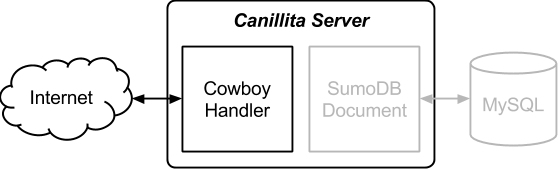
\includegraphics[width=.9\textwidth]{img/arch-web.png}}
\only<3>{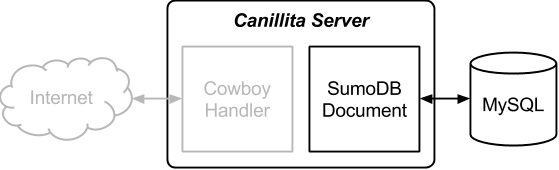
\includegraphics[width=.9\textwidth]{img/arch-db.png}}
\begin{itemize}
	\item<+-> \texttt{canillita} es una applicaci\'on Erlang t\'ipica
	\item<+-> Usa \texttt{cowboy} como web framework
	\item<+-> Y \texttt{sumo\_db} como motor de persistencia
\end{itemize}
\end{frame}

\subsection{Componentes}
\begin{frame}[t]{Cowboy Handler}
\alert{\texttt{canillita\_news\_handler}}
\begin{itemize}
	\item Procesa requests \texttt{HTTP}
	\item Responde a \texttt{POST /news} utilizando un \textbf{REST handler}
	\item Responde a \texttt{GET /news} utilizando un \textbf{Loop handler}
\end{itemize}
~\\ \only<2>{
En la funci\'on \texttt{init} se determina qu\'e handler utilizar:
\handlerinit
}
\end{frame}

\begin{frame}[t]{Rest Handler}
\begin{itemize}
	\item \texttt{cowboy\_rest} define m\'ultiples funciones a implementar para procesar un request
	\item s\'olo se implementan las que se necesitan
	\item en nuestro caso:
\end{itemize}
~\\ \only<2>\restcallbacks
\only<3>\restcallbacksa
\end{frame}

\begin{frame}[t]{Rest Handler}
{La funci\'on \texttt{handle\_post}}
\only<1>{\handlepost}
\only<2>{\handleposta Obtiene el \emph{body} del request}
\only<3>{\handlepostb Lo parsea como JSON}
\only<4>{\handlepostc Extrae los campos \texttt{title} y \texttt{content}}
\only<5>{\handlepostd Crea y almacena la noticia}
\only<6>{\handleposte La env\'ia a quienes est\'en escuchando}
\only<7>{\handlepostf Devuelve \texttt{204 No Content}}
\end{frame}

\begin{frame}{Loop Handler}
\begin{itemize}
	\item en nuestro handler, desde \texttt{init} estamos llamando a \texttt{handle\_get}
	\item m\'as all\'a de \texttt{init}, \texttt{cowboy\_req} define una \'unica funci\'on para implementar un \emph{loop handler}: \texttt{info}
	\item es llamada cada vez que el proceso recibe un mensaje
\end{itemize}
\end{frame}

\begin{frame}[t]{Loop Handler}
{La funci\'on \texttt{handle\_get}}
\only<1>{\handleget}
\only<2>{\handlegeta Setea el encoding y comienza a responder}
\only<3>{\handlegetb Obtiene las noticias de la base de datos}
\only<4>{\handlegetc Env\'ia cada una de ellas usando la funci\'on \texttt{send\_flash}}
\only<5>{\handlegetd Se subscribe para recibir futuras noticias}
\only<6>{\handlegete y se queda esperando mensajes, que llegar\'an a \texttt{info}}
\end{frame}

\begin{frame}[t]{Loop Handler}
{Otras funciones}
\only<1>{\infosend}
\only<2>{\infosenda La funci\'on \texttt{info}, env\'ia la noticia}
\only<3>{\infosendb y vuelve a esperar mensajes}
\only<4>{\infosendc La funci\'on \texttt{send\_flash} extrae los campos de la noticia}
\only<5>{\infosendd compone un bloque de texto a enviar}
\only<6>{\infosende y lo env\'ia al cliente}
\only<7>{\infosendf La funci\'on \texttt{notify} recorre la lista de subscriptos}
\only<8>{\infosendg y le env\'ia un mensaje a cada uno}
\end{frame}

\begin{frame}{SumoDB Document}
\alert{\texttt{canillita\_news}}
\begin{itemize}
	\item Implementa el behaviour \texttt{sumo\_doc}
	\item Encapsula estado y comportamiento del modelo \textbf{News}
	\item Administra su persistencia a trav\'es de \emph{SumoDB}
\end{itemize}
\pause
~\\
El behaviour \texttt{sumo\_doc} define tres funciones a implementar:
\begin{itemize}
	\item\texttt{sumo\_schema}: definici\'on del modelo
	\item\texttt{sumo\_sleep}: traducci\'on al formato de \emph{SumoDB}
	\item\texttt{sumo\_wakeup}: traducci\'on a nuestro formato
\end{itemize}
\end{frame}

\begin{frame}{Canillita News}
{Behaviour Callbacks}
\canillitanews
\end{frame}

\begin{frame}[t]{Canillita News}
{Otras funciones}
\only<1>{\canillitanewsother}
\only<2>{\canillitanewsothera La funci\'on \texttt{new}, crea una entidad y la persiste}
\only<3>{\canillitanewsotherb Las funciones \texttt{get\_*} son simples proyectores}
\only<4>{\canillitanewsotherc La funci\'on \texttt{latest\_news} retorna todos las entidades}
\end{frame}

\section{Benchmarks}
\subsection{Herramientas}
\begin{frame}{Tsung}
\center{
\includegraphics[height=0.25\textheight]{img/tsung-logo.png}}
	\begin{itemize}
		\item \href{http://tsung.erlang-projects.org/}{http://tsung.erlang-projects.org/}
		\item<+-> Herramienta de medici\'on de carga multi-protocolo distribuida
		\item<+-> Hecha en Erlang
		\item<+-> Puede utilizarse tambi\'en para testear
	\end{itemize}
\end{frame}

\subsection{Resultados}
\begin{frame}{Escenario}
	\begin{description}
		\item[Test]\begin{itemize}
			\item Duraci\'on: 500 segundos
			\item Requests a \texttt{POST /news}: 1 por segundo
			\item Requests a \texttt{GET /news}: 50 por segundo
		\end{itemize}
		\item[Hardware]\begin{itemize}
			\item MacBook PRO con OSX 10.9
			\item Procesador: 2.4 GHz Intel Core i5
			\item Memoria: 8 GB 1600 MHz DDR3
		\end{itemize}
	\end{description}

\end{frame}

\begin{frame}[t]{Usuarios conectados}
\center{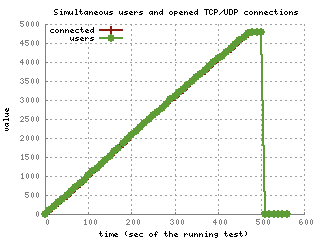
\includegraphics[height=.7\textheight]{img/graphes-simultaneous-users.png}} \\
Un servidor \emph{b'asico} soporta m\'as de 4500 conexiones
\end{frame}

\begin{frame}[t]{Status Codes}
\center{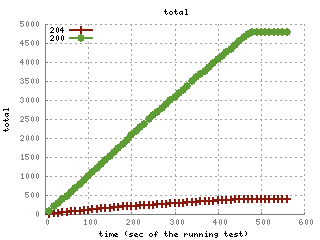
\includegraphics[height=.7\textheight]{img/graphes-http_code.png}} \\
Todos los requests se procesan exitosamente
\end{frame}

\appendix

\begin{frame}{Moraleja}

	\emph{Erlang} es un lenguaje complejo, no es sencillo dominarlo r\'apidamente. \pause Sin embargo, para ciertos escenarios habituales no resulta dif\'icil construir las aplicaciones necesarias e integrarlas con otros sistemas sin conocer el lenguaje a fondo. \\
	\pause Y esas aplicaciones traen \emph{gratis} todas las ventajas de Erlang, como \emph{supervisi\'on de procesos}, \emph{manejo de m\'ultiples nodos}, etc. \\
	\pause Adem\'as, con ese punto de partida, se puede continuar aprendiendo el lenguaje paso a paso.
	
\end{frame}

\begin{frame}{Materiales}
	\begin{description}
		\item[Sobre m\'i]~\\
			\begin{itemize}
				\item Soy \textbf{\href{http://twitter.com/elbrujohalcon}{@elbrujohalcon}} en Twitter
				\item Soy \href{http://github.com/elbrujohalcon}{elbrujohalcon} en GitHub
			\end{itemize}
		\item[Sobre Inaka]~\\
			\begin{itemize}
				\item Pueden ver nuestro sitio web: \href{http://inaka.net}{http://inaka.net}
				\item Y nuestro Blog: \href{http://inaka.net/blog}{http://inaka.net/blog}
			\end{itemize}
		\item[Sobre Canillita]~\\
			\begin{itemize}
				\item El c\'odigo est\'a en GitHub: \textbf{\href{https://github.com/inaka/canillita}{inaka/canillita}}
				\item Las slides tambi\'en: \textbf{\href{https://github.com/inaka/talks}{inaka/talks}}
			\end{itemize}
	\end{description}
\end{frame}

\begin{frame}
	\begin{center}
		{\Huge Muchas Gracias!}
	\end{center}
\end{frame}

\end{document}